\documentclass[tikz,14pt,border=10pt]{standalone}
\usepackage{amsmath}
\usepackage{textcomp}
\usetikzlibrary{shapes,arrows}
\begin{document}
% Definition of blocks:
\tikzset{%
  block/.style    = {draw, rectangle, minimum height = 2cm,
    minimum width = 2cm, node distance = 3.5cm},
  sum/.style      = {draw, circle, node distance = 3.5cm}, % Adder
  input/.style    = {coordinate}, % Input
  output/.style   = {coordinate} % Output
}
% Defining string as labels of certain blocks.
\newcommand{\suma}{\Large$+$}
\newcommand{\inte}{$\displaystyle \int$}
\newcommand{\derv}{\huge$\frac{d}{dt}$}
\newcommand{\DWT}{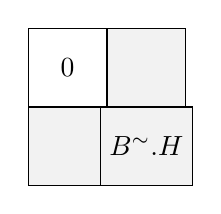
\begin{tikzpicture}%
    \draw node [draw, minimum width = 1cm, minimum height = 1cm] (0) {$0$};
    \draw node [draw, minimum width = 1cm, minimum height = 1cm, node distance = 1cm, right of=0, fill=gray!10] (empty) {};
    \draw node [draw, minimum width = 1cm, minimum height = 1cm, node distance = 1cm, below of=0, fill=gray!10] {};
    \draw node [draw, minimum width = 1cm, minimum height = 1cm, node distance = 1cm, below of=empty, fill=gray!10] {$B^\sim.H$};
    %\draw grid[very thick] (2,2);
    %\draw node (L) at (0.5,1.5) {$0$};
    %\draw node (H) at (1.5,0.5) {$B^\sim.H$};
  \end{tikzpicture}
}

\begin{tikzpicture}[auto, >=triangle 45]

  \draw
  node [block] (AL) {$[A.L]$}
  node [block, right of=AL] (DWTA) {$\{A.L, A.H\}$}
  node [block, right of=DWTA] (BL) {$[B.L]$}
  node [block, right of=BL] (DWTB) {$\{B.L, B.H\}$}
  node [block, right of=DWTB] (CL) {$[C.L]$}
  node [block, right of=CL] (DWTC) {$\{C.L, C.H\}$}
  node [block, above of=DWTA] (A) {$A$}
  node [block, above of=DWTB] (B) {$B$}
  node [block, above of=DWTC] (C) {$C$}
  node [block, below of=DWTA] (AH) {$[A.H]$}
  node [block, below of=DWTB] (BH) {$[B.H]$}
  node [block, below of=DWTC] (CH) {$[C.H]$}
  node [block, below of=AH] (BHA) {$[B_A.H]$}
  node [sum, below of=BH] (suma) {\suma}
  node [block, below of=CH] (BHC) {$[B_C.H]$}
  node [draw, thick, rectangle, right of=BHA, node distance=3.5cm] (12a) {$1/2$}
  node [draw, thick, rectangle, left of=BHC, node distance=3.5cm] (12b) {$1/2$}
  node [block, below of=suma] (BHp) {$[B^{\sim}.H]$}
  node [node distance=3.5cm, below of=BHp] {\DWT}
  ;
  
  \draw [->] (A) -- node {DWT} (DWTA);
  \draw [->] (DWTA) -- node {iDWT} (AL);
  \draw [->] (B) -- node {DWT} (DWTB);
  \draw [->] (DWTB) -- node {iDWT} (BL);
  \draw [->] (C) -- node {DWT} (DWTC);
  \draw [->] (DWTC) -- node {iDWT} (CL);
  \draw [->] (DWTA) -- node {iDWT} (AH);
  \draw [->] (DWTB) -- node {iWDT} (BH);
  \draw [->] (DWTC) -- node {iWDT} (CH);
  \draw [->] (AH) -- node {$[B.L]\rightarrow [A.L]$} (BHA);
  \draw [->] (BH) -- (suma);
  \draw [->] (CH) -- node {$[B.L]\rightarrow [C.L]$} (BHC);
  \draw [->] (BHA) -- (12a);
  \draw [->] (BHC) -- (12b);
  \draw [->] (12a) -- (suma);
  \draw [->] (12b) -- (suma);
  \draw [->] (suma) -- (BHp);
  
\end{tikzpicture}
\end{document}


	% Drawing the blocks of first filter :
	node at (0,0)[right=-3mm]{\Large \textopenbullet}
	node [input, name=input1] {} 
	node [sum, right of=input1] (suma1) {\suma}
	node [block, right of=suma1] (inte1) {\inte}
         node at (6.8,0)[block] (Q1) {\Large $Q_1$}
         node [block, below of=inte1] (ret1) {\Large$T_1$}

    % Joining blocks. 
    % Commands \draw with options like [->] must be written individually
	\draw[->](input1) -- node {$X(Z)$}(suma1);
 	\draw[->](suma1) -- node {} (inte1);
	\draw[->](inte1) -- node {} (Q1);
	\draw[->](ret1) -| node[near end]{} (suma1);
	% Adder
\draw
	node at (5.4,-4) [sum, name=suma2] {\suma}
    	% Second stage of filter 
	node at  (1,-6) [sum, name=suma3] {\suma}
	node [block, right of=suma3] (inte2) {\inte}
	node [sum, right of=inte2] (suma4) {\suma}
	node [block, right of=suma4] (inte3) {\inte}
	node [block, right of=inte3] (Q2) {\Large$Q_2$}
	node at (9,-8) [block, name=ret2] {\Large$T_2$}
;
	% Joining the blocks of second filter
	\draw[->] (suma3) -- node {} (inte2);
	\draw[->] (inte2) -- node {} (suma4);
	\draw[->] (suma4) -- node {} (inte3);
	\draw[->] (inte3) -- node {} (Q2);
	\draw[->] (ret2) -| (suma3);
	\draw[->] (ret2) -| (suma4);
         % Third stage of filter:
	% Defining nodes:
\draw
	node at (11.5, 0) [sum, name=suma5]{\suma}
	node [output, right of=suma5]{}
	node [block, below of=suma5] (deriv1){\derv}
	node [output, right of=suma5] (sal2){}
;
	% Joining the blocks:
	\draw[->] (suma2) -| node {}(suma3);
	\draw[->] (Q1) -- (8,0) |- node {}(ret1);
	\draw[->] (8,0) |- (suma2);
	\draw[->] (5.4,0) -- (suma2);
	\draw[->] (Q1) -- node {}(suma5);
	\draw[->] (deriv1) -- node {}(suma5);
	\draw[->] (Q2) -| node {}(deriv1);
    	\draw[<->] (ret2) -| node {}(deriv1);
    	\draw[->] (suma5) -- node {$Y(Z)$}(sal2);
    	% Drawing nodes with \textbullet
\draw
	node at (8,0) {\textbullet} 
	node at (8,-2){\textbullet}
	node at (5.4,0){\textbullet}
    	node at (5,-8){\textbullet}
    	node at (11.5,-6){\textbullet}
    	;
	% Boxing and labelling noise shapers
	\draw [color=gray,thick](-0.5,-3) rectangle (9,1);
	\node at (-0.5,1) [above=5mm, right=0mm] {\textsc{first-order noise shaper}};
	\draw [color=gray,thick](-0.5,-9) rectangle (12.5,-5);
	\node at (-0.5,-9) [below=5mm, right=0mm] {\textsc{second-order noise shaper}};
